\documentclass[10pt,oneside,a4paper,final,english]{memoir}

\usepackage{palatino}
\usepackage{microtype}
\usepackage{lscape}
\usepackage{multicol}
%\usepackage{epic,eepic}
\usepackage{latexsym}
\usepackage{verbatim}
\usepackage{listings}
\usepackage{ulem}
\usepackage{hyperref}

\let\footruleskip\undefined
\usepackage{fancyhdr}
\usepackage[final]{fixme}

\let\fref\undefined
\usepackage[plain]{fancyref}

%% FOR LOOP
\usepackage{ifthen,calc}
\newcounter{myforloopcounter}
\newcommand{\forloop}[5][1]% 
{\setcounter{#2}{#3}% 
\ifthenelse{#4}% 
{#5%
  \addtocounter{#2}{#1}% 
  \forloop[#1]{#2}{\value{#2}}{#4}{#5}% 
}%
% Else 
{}%
}% 


%% USAGE
%\forloop[step]{counter}{initial_value}{conditional}{code_block} 
\input{env/languages}
\usepackage[pdftex]{graphicx}

\DeclareGraphicsExtensions{.jpg .png .pdf}


\usepackage{amsmath}
\usepackage{latexsym}
\usepackage{amssymb}


\usepackage[osf,sc]{mathpazo}
\usepackage{microtype}
%\usepackage{fourier}
\linespread{1.05}

%\usepackage[charter]{mathdesign}
%\usepackage{lmodern}

%\usepackage{algorithmic}
%\usepackage{algorithm}

\usepackage{amsthm}


\theoremstyle{plain}  \newtheorem{definition}{Definition}
\theoremstyle{remark} \newtheorem{lemma}{Lemma}
\theoremstyle{plain}  \newtheorem{theorem}{Theorem}
\theoremstyle{remark}  \newtheorem{example}{Example}


\newcommand{\p}{\ensuremath{^\prime}}
\DeclareGraphicsExtensions{.jpg, .eps, .png}
%%% Local Variables:
%%% mode: plain-tex
%%% TeX-master: "../master"
%%% End:

\usepackage{algorithmic}
\usepackage{algorithm}
\usepackage[sectionbib,square]{natbib}
%\bibpunct{(}{)}{,}{a}{}{}
\setcitestyle{alpha}
%\setcitestyle{numbers,aysep={},yysep={;}}

\usepackage{datetime}

\chapterstyle{thatcher}

\setcounter{secnumdepth}{0}
\setcounter{tocdepth}{0}




%\pagestyle{fancy}
\begin{document}
  \fontencoding{T1}
%  \fontseries{m}
%  \fontshape{n}
%  \fontsize{12}{15}
%  \selectfont


%%%%%%%%%%%%%%%%%%%%%%%%%%%%%%%%%%%%%%%%%%%%%%%%%%%%%%%%
%                    Forside
%%%%%%%%%%%%%%%%%%%%%%%%%%%%%%%%%%%%%%%%%%%%%%%%%%%%%%%%
\makeatletter % open mode for reading @ signed variables
\def\maketitle{%
 \null
 \thispagestyle{empty}%
 \vfill
 \begin{center}\leavevmode
   \normalfont
   \LARGE{\raggedleft \@title\par}%
   \hrulefill\par
   \large{\raggedleft \subtitle\par}%
   \vskip 2cm
   {\today\par}%
 \end{center}%
 \vfill
 \begin{flushleft}
   {\large \@author } \\
   {\footnotesize \suplementInfo }
 \end{flushleft}
 \clearpage % Terminates the page here. Everything else vil be placed
            % on next page.
}
\makeatother % closing mode for reading @ signed variables
%%%%%%%%%%%%%%%%%%%%%%%%%%%%%%%%%%%%%%%%%%%%%%%%%%%%%%%%
%               Data til forside
%%%%%%%%%%%%%%%%%%%%%%%%%%%%%%%%%%%%%%%%%%%%%%%%%%%%%%%%
\title{Complementarity Problems $\cdot$ Week VI}

\def\subtitle{CCO $\cdot$ Constraint Continous Optimization}

\author{Johan Sejr Brinch Nielsen} \def\suplementInfo{

\kern 5pt \hrule width 11pc \kern 5pt

\begin{tabular}{ll}
Email: & zerrez@diku.dk  \\
Cpr.:  & 260886-2547
\end{tabular}

% putter 5pt spacing oven over og neden under stregen
\kern 5pt \hrule width 11pc \kern 5pt

Dept. of Computer Science,  \\
University of Copenhagen

}


\maketitle
\newpage

\section{Introduction}
In this week assignment, the optimization problem is expanded with
equality and inequality contains. The goal is the implement at
modified version of one of the previous optimization methods, that can
handle these new constraints.


\section{Constrained Optimization}
The unconstrained optimization problem is formalized as:
\[
\min f(x)
\]
Where $x$ is free to take any value in $\mathbb{R}^n$.

By introducing equality and inequality constrains, this problem is
expanded to:
\begin{center}\begin{tabular}{rll}
min & $f(x)$ & \\
subject to & $c_i(x) = 0$    & for $i \in E$\\
           & $c_i(x) \geq 0$ & for $i \in I$
\end{tabular}\end{center}

Where $E$ is the set of equality constraint indexes, while $I$ is the
set of inequality constraint indexes. $c_i(x)$ is the $i$th
constraint applied to vector $x$.

It is possible to solve an optimization problem with only equality
constraints, by approximating $f(x)$ with the lagrangian
$L(x,\lambda)$. This yields a quadratic function which can be
solved by finding $x^*$ and $\lambda^*$ that fulfills the
Karush-Kuhn-Tucker conditions, which are necessary conditions for a
minimum.


\section{Active Set Methods}
Active set methods is a way of solving problems with inequality
constraints by transforming them into problems with equality
constraints only.

Consider again problems the general constrained optimization problem:
\begin{center}\begin{tabular}{rll}
min & $f(x)$ & \\
subject to & $c_i(x) = 0$    & for $i \in E$\\
           & $c_i(x) \geq 0$ & for $i \in I$
\end{tabular}\end{center}

The idea of active set methods is to only consider inequality
constraints that are being violated - the active
constraints. When an inequality constraint is active, it is
represented by an equality constrained forcing its value to zero. This
is formalized as:
\begin{center}\begin{tabular}{rll}
min & $f(x)$ & \\
subject to & $c_i(x) = 0$    & for $i \in E$\\
           & $c_i(x) = 0$ & for $i \in W_k$
\end{tabular}\end{center}
Where $W_k$ are the active inequality constraints in the $k$th
iteration.

One of the simpler ways to keep track of active and nonactive
inequality constraints, is to simply add a constraint to the active
set whenever it is violated. When the chosen direction is going to
violate constraint $j$ we enforce it. This will make the approximation
follow the constraint border.

Whenever an inequality constraint is not violated it is not part of
the active set. There is no reason to enforce a constraint that is far
away. Intuitively, this approach can be thought of as letting the
optimization loose until it brakes the rules. When a rule is broken we
enforce it.


\section{Gradient-Project Method}
In the specific problem of this weeks programming case, we are to
implement upper and lower bounds on the angles between each arm. This
specific inequality constraint has the interesting property that it
can be tested on each angle individually. It categorizes as a ``box''
constraint.

The Gradient-Project method specializes in precisely this kind of
constraints. The method uses the negative gradient $-g$ as its
direction (just as the gradient descent). If one or more constraints
are violated, the direction vector is projected onto one or more
constraint lines, to ease the constraints; the violated constraints
are added to the active set and enforced. Since this changes the
direction of the step, it is necessary to test whether a better
objective value is found in the new point. If not, the point is
rejected and the step size lowered. If so, the point is accepted and a
new iteration begins.

Assuming that the first point is located in the feasible region, the
method will always be able to find a better objective value inside the
feasible region. There must exist some step size small enough to yield
a point inside the feasible region together with a better objective
value. The last fact is due to the use of the negative gradient as
direction.

In the implementation, any starting point outside the feasible region
will be moved inside the region if no feasible point is found in the
search direction.

The process of projection is implemented using $\max$ and $\min$
functions on each angle individually. This restricts each angles to be
within the given interval. The angles are normalized to the interval
$[-\pi; \pi]$, before the constraints are enforced. Without
normalization many of the angles will hit either the upper or lower
bound, even though they are in fact inside the interval.


\section{Verification}
Verification has been performed using 20 angles. I have chosen to
increase the number of angles, because it makes it more clear how the
constraints effects the solution.

Instead of making several plots, I have made four movies with 75
frames each. I can recommend watching these with a player that
supports control over the movie speed (frame per second). The
following mplayer invocation works very well:
\begin{verbatim}
mplayer -fps 1 themovie.mpg
\end{verbatim}

All movies shows the same optimization problem, but under different
conditions. In each movie, the constraints on the angles are adjusted
between each frame by the following term:
\[ -\frac{\pi}{i} \leq \theta \leq \frac{\pi}{i} \]

Where $i$ is the current frame. Hence, the angles are squeezed from
the full circle interval $[-\pi; \pi]$ to $[-\pi/75; \pi/75]$.

Due to technical problems, the movies are malformed. The scale is
wrong. They look flat, but are in fact $[-12; 2]$ in the $x$ axis and
$[0 12]$ in the $y$ axis. Due to another technical problem, no axis
are shown in the movies.

In the movies, the goal is not always reached. I can find two possible
reasons for this:
\begin{enumerate}
\item The number of iterations are too low. I run each approximation
  in at most 200 iterations. If the initial guess is too far from the
  goal this could lead to a result far from the goal.
\item The unconstrained optimization runs directly into a constraint
  line without changing direction (step size equals zero).
\end{enumerate}


\subsection{Movie 1 - zero free angles}
In this movie all angles are affected by the constraints equally and
hence, none of them can be chosen freely.

The interesting part in this movie is to see how the arm bends while
the constraints tightens in. In the end the angles are too small for
the arm to reach the goal. Instead it shoots over, as is seen in the
following image:
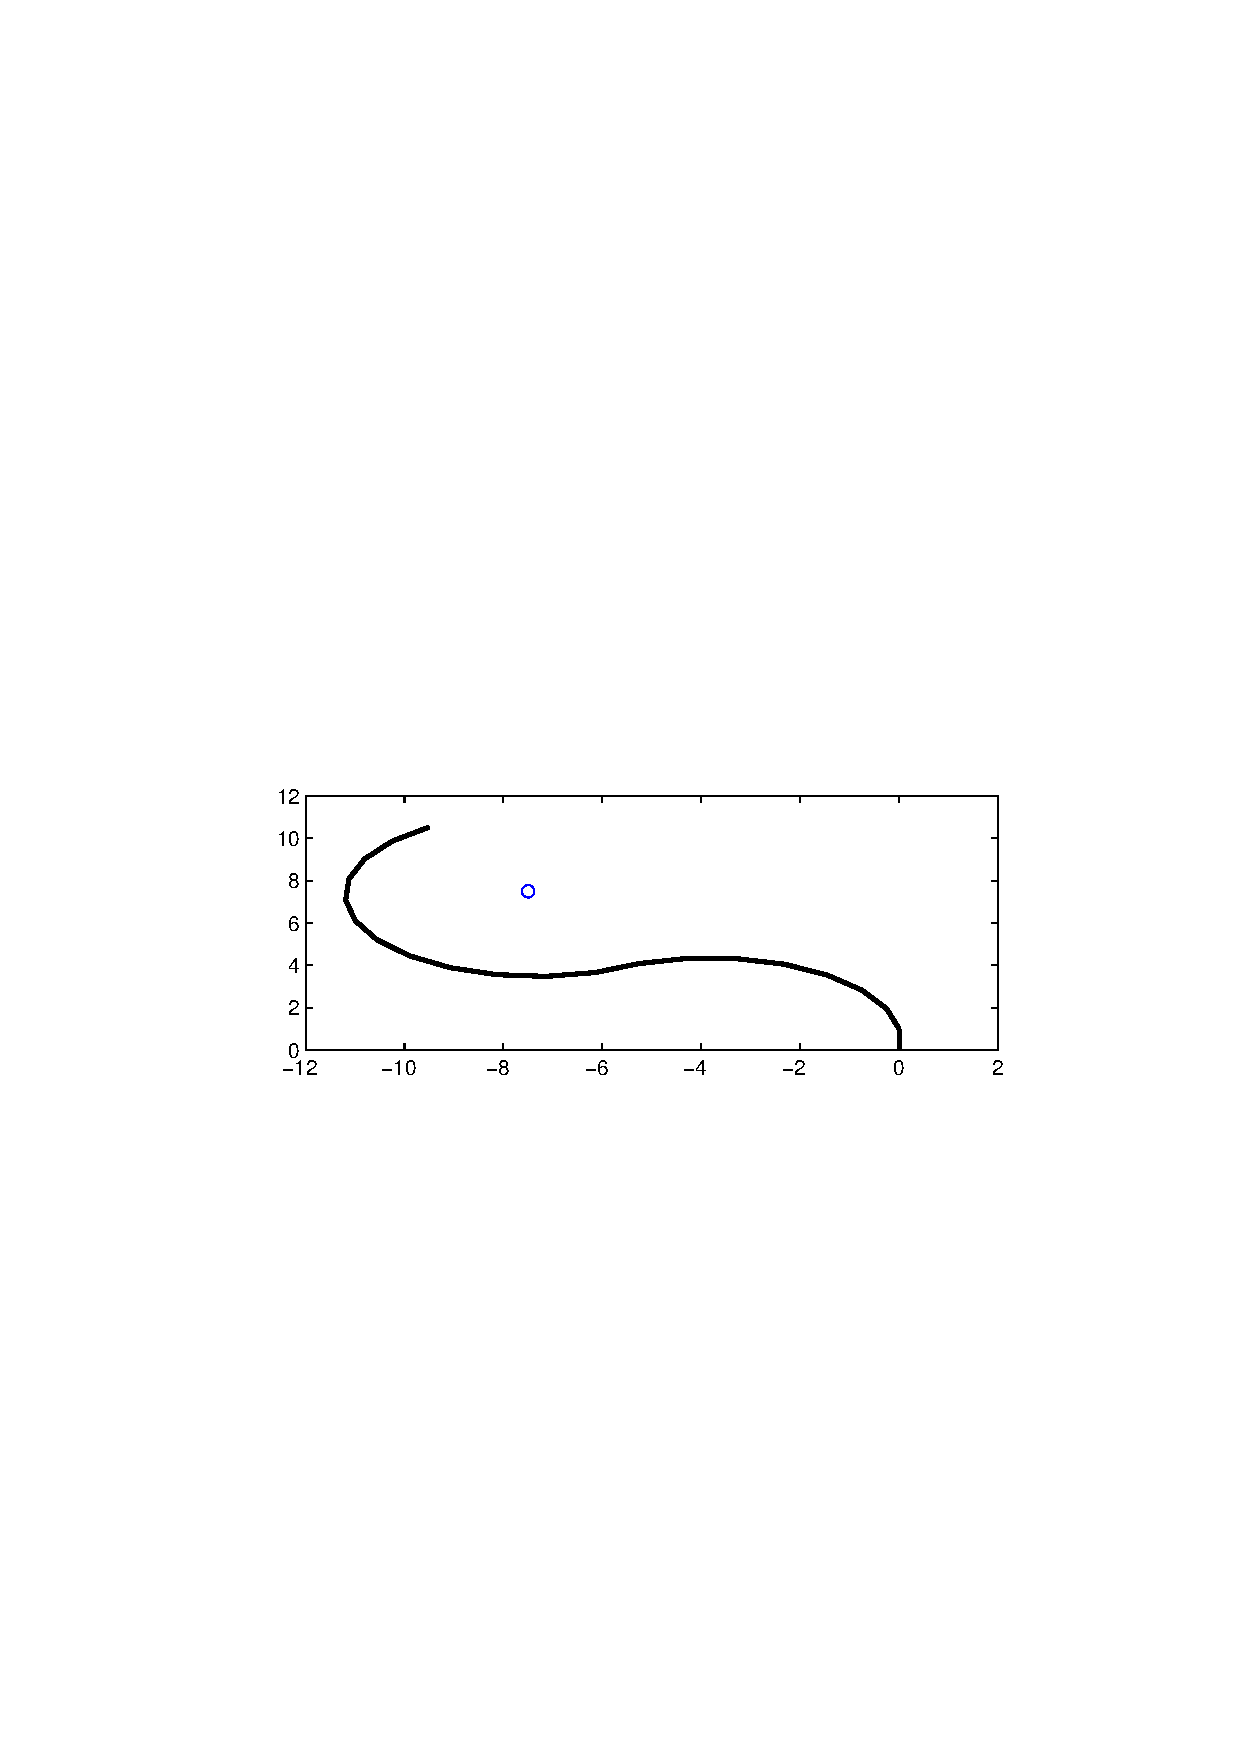
\includegraphics[width=\textwidth]{images/movie1.pdf}

\subsection{Movie 2 - one free angle}
In this movie angle number 10 is unaffected of the constraints and can
therefore be chosen freely.

Here, the interesting part is to see how the optimization exploits
this in its attempt to reach the goal.

An example of such a ``crack'' is clearly visible in the image below:\\
\includegraphics[width=\textwidth]{images/movie2.pdf}

\subsection{Movie 3 - two free angles}
In this movie angles number 5 and 10 are unaffected of the constraints
and can hence be chosen freely.

Here, the interesting part is to see how these two free angles can be
used in cooperation to find a path to the goal.

An example of both angles being used in a ``free'' matter is shown
below:\\
\includegraphics[width=\textwidth]{images/movie3.pdf}

\subsection{Movie 4 - three free angles}
In this movie angles number 5, 10 and 15 are unconstrained.  This
allows for three possible ``cracks''. An example of such three
``crakcs'' are shown here:\\

\includegraphics[width=\textwidth]{images/movie4.pdf}

\section{Conclusion}
I have implemented and described the Gradient-Project method and shown
how different inequality constraints affects the solutions found. Both
with wide angles moving to small angles and with several free angles.

Unfortunately the Gradient-Project method only works on ``box''
constraints, where each constraint can be tested against each variable
individually.


\section{Source Code}
This section contains the MatLab code for the Gradient-Projection
implementation. I have also added a function for generating movies.

\subsection{Gproject}
\verbatiminput{../code/gproject.m}

\subsection{Gproject Backtrack}
\verbatiminput{../code/gproject_backtrack.m}

\subsection{Gproject Movie}
\verbatiminput{../code/gproject_movie.m}

\end{document}

%%% Local Variables:
%%% mode: latex
%%% TeX-master: t
%%% End:
